\documentclass[journal]{IEEEtran}

% Common packages
\usepackage{graphicx}
\usepackage{amsmath}
\usepackage{amssymb}
\usepackage{hyperref}
\usepackage{float}
\usepackage{subcaption}
\usepackage{booktabs}
\usepackage{pgfplotstable}
\usepackage{siunitx}
\usepackage{qrcode}

\pgfplotsset{compat=1.18}
\sisetup{separate-uncertainty=true}
\pgfplotstableset{
    col sep=comma,
    every head row/.style={before row=\toprule, after row=\midrule},
    every last row/.style={after row=\bottomrule},
}

\begin{document}

% ---------- TITLE & AUTHOR ----------
\title{06-FINE STRUCTURE of TWO-ELECTRON ATOM He}
\author{IBRAHIM H.I. ABUSHAWISH \\
Istanbul University, Department of Physics \\
Instructor: \\
Experiment Date: November 17, 2026 , Report Submission Date: \\
Course \& Section Number: PHYS4704}

\markboth{Physics Laboratory Reports}{2026}

\maketitle

% ---------- ABSTRACT ----------
\begin{abstract}
The visible emission spectrum of the two-electron helium atom (He I) was investigated using a goniometer-mounted diffraction grating spectrometer with an accepted manual grating constant of $d_{\text{manual}} = \SI{1684.0}{\nano\meter}$. Five first-order ($m = 1$) spectral lines were measured on both left and right sides of the recorded zero-order angle $\theta_0 = \SI{110.0}{\degree}$, yielding average diffraction angles $\theta_{\text{ave}}$ of $\SI{25.95}{\degree}$ (red), $\SI{23.20}{\degree}$ (yellow), $\SI{20.25}{\degree}$ (green), $\SI{17.60}{\degree}$ (blue), and $\SI{15.50}{\degree}$ (purple). Using $d_{\text{manual}} = \SI{1684.0}{\nano\meter}$, the corresponding wavelengths are $\SI{736.9 \pm 1.9}{\nano\meter}$, $\SI{663.4 \pm 1.9}{\nano\meter}$, $\SI{582.9 \pm 1.9}{\nano\meter}$, $\SI{509.2 \pm 2.0}{\nano\meter}$, and $\SI{450.0 \pm 2.0}{\nano\meter}$, exhibiting a uniform positive shift of $\overline{\Delta\lambda} = \SI{69.24}{\nano\meter}$ (mean relative error \SI{13.66}{\percent}) relative to the accepted manual transitions in the parahelium singlet ($3\,^{1}D \rightarrow 2\,^{1}P$ at $\SI{667.8}{\nano\meter}$, $4\,^{1}S \rightarrow 2\,^{1}P$ at $\SI{504.8}{\nano\meter}$) and orthohelium triplet ($3\,^{3}D \rightarrow 2\,^{3}P$ at $\SI{587.6}{\nano\meter}$, $4\,^{3}D \rightarrow 2\,^{3}P$ at $\SI{447.1}{\nano\meter}$, $3\,^{3}P \rightarrow 2\,^{3}S$ at $\SI{388.9}{\nano\meter}$) systems. Inverting the manual grating equation with the reference wavelengths gave line-by-line grating constants $d_i$ from $\SI{1455.3}{\nano\meter}$ to $\SI{1526.1}{\nano\meter}$, with a mean of $\bar{d} = \SI{1482.0 \pm 12.9}{\nano\meter}$ ($s_d = \SI{28.8}{\nano\meter}$, \SI{11.99}{\percent} below $d_{\text{manual}}$). Re-evaluating the wavelengths with $\bar{d}$ reduced the mean relative error against the accepted manual wavelengths to \SI{1.44}{\percent} (maximum \SI{2.89}{\percent}). Ordinary least-squares regression of the $m = 1$ calibration curve ($\lambda_{\text{lit}}$ versus $\sin\theta_{\text{ave}}$) yielded a slope of $d_{\text{cal}} = \SI{1617.1 \pm 52.3}{\nano\meter}$ (\SI{3.97}{\percent} below $d_{\text{manual}}$), an intercept of $\SI{-45.9 \pm 18.6}{\nano\meter}$, and $R^2 = 0.9969$, while a zero-intercept fit gave $d_{\text{eff}} = \SI{1489.8 \pm 13.6}{\nano\meter}$ (\SI{11.53}{\percent} below $d_{\text{manual}}$).
\end{abstract}

% ---------- INTRODUCTION ----------
\section{Introduction}
Optical atomic spectroscopy provides direct experimental access to the quantized electronic energy structure of atoms. Whereas the single-electron hydrogen atom can be solved analytically and exhibits energy levels that depend primarily on the principal quantum number $n$, multi-electron atoms introduce inter-electronic Coulomb repulsion, shielding of the nuclear charge, and quantum-mechanical exchange symmetry arising from the Pauli exclusion principle. The neutral helium atom (He I), containing two electrons bound to a nucleus of charge $Z = 2$, serves as the simplest physical prototype for two-electron quantum mechanics.

Because the total two-electron wavefunction must be antisymmetric under particle exchange, the spin configuration partitions the excited energy states of helium into two distinct term manifolds: parahelium, characterized by antiparallel electron spins forming singlet states ($S = 0$), and orthohelium, characterized by parallel spins forming triplet states ($S = 1$) \cite{lab_manual, haken_wolf}. Electric dipole selection rules forbid radiative transitions between states of different spin multiplicity ($\Delta S = 0$), causing parahelium and orthohelium to behave spectroscopically as two non-combining level systems. Furthermore, magnetic spin-orbit coupling splits triplet levels with $L > 0$ into closely spaced fine-structure multiplets characterized by total angular momentum $J$.

In this experiment, the visible emission spectrum of a helium discharge lamp was dispersed using a diffraction grating spectrometer. The objectives were to measure the first-order ($m = 1$) left and right diffraction angles of the visible spectral lines, calculate experimental wavelengths via the grating equation using the manual grating constant, determine the experimental grating constant directly from the helium reference spectrum and the $m = 1$ calibration curve, and compare all results with the accepted laboratory manual values.

% ---------- THEORY ----------
\section{Theory}

\subsection{Two-Electron Hamiltonian and Spin-Orbit Coupling}
In the ground state of the helium atom, both $1s$ electrons occupy the $n = 1$ shell ($1s^2$). In singly excited states, one electron remains in the $1s$ orbital ($n_1 = 1$, $l_1 = 0$) while the second electron is promoted to an upper orbital ($n_2 > 1$, $l_2 = 0, 1, \dots, n_2 - 1$). The stationary energy eigenvalues $E$ of an $N$-electron atom satisfy the time-independent Schr\"odinger equation:
\begin{equation}
    H \Psi(\mathbf{r}_i) = E \Psi(\mathbf{r}_i)
    \label{eq:schrodinger}
\end{equation}
where $\Psi(\mathbf{r}_i)$ is the multi-electron wavefunction and $H$ is the total Hamiltonian operator. Because the inter-electronic electrostatic repulsion breaks spherical symmetry for individual electrons, Equation~\eqref{eq:schrodinger} cannot be solved in closed analytical form and requires perturbative or variational approximations \cite{lab_manual}.

An electron orbiting in the nuclear electric field experiences an effective internal magnetic field $\mathbf{B}$ proportional to its orbital angular momentum $\mathbf{l}$. The interaction between the electron's spin magnetic moment $\boldsymbol{\mu}_s$ and this internal field contributes a spin-orbit orientational energy $E_{nl}$:
\begin{equation}
    E_{nl} = -\boldsymbol{\mu}_s \cdot \mathbf{B} = \zeta\,\mathbf{s} \cdot \mathbf{l}
    \label{eq:spin_orbit}
\end{equation}
where $\zeta$ is the fine-structure constant parameterizing the spin-orbit coupling strength. Including kinetic energy, nuclear Coulomb attraction, pairwise electron-electron repulsion, and spin-orbit interaction yields the multi-electron atomic Hamiltonian:
\begin{equation}
\begin{aligned}
    H &= \sum_{i=1}^{N} \left(-\frac{\hbar^2}{2 m_e} \nabla_i^2 - \frac{Z e^2}{4 \pi \varepsilon_0 r_i}\right) \\
      &\quad + \sum_{j > i = 1}^{N} \frac{e^2}{4 \pi \varepsilon_0 r_{ij}} + \sum_{i=1}^{N} \zeta_i(r_i)\,\mathbf{s}_i \cdot \mathbf{l}_i
\end{aligned}
    \label{eq:hamiltonian}
\end{equation}
where $m_e$ is the electron mass, $Z$ is the atomic number, $r_i$ is the radial coordinate of the $i$-th electron, and $r_{ij} = |\mathbf{r}_i - \mathbf{r}_j|$ is the inter-electronic separation.

\subsection{Russell-Saunders (\texorpdfstring{$LS$}{LS}) Coupling, Parahelium, and Orthohelium}
In light atoms such as helium, the electrostatic interaction among the outer electrons dominates over individual spin-orbit couplings, so Russell-Saunders ($LS$) coupling applies. The individual orbital and spin angular momenta couple separately into total orbital and total spin vectors:
\begin{equation}
    \mathbf{L} = \sum_i \mathbf{l}_i, \qquad \mathbf{S} = \sum_i \mathbf{s}_i
    \label{eq:LS_sums}
\end{equation}
which subsequently combine to form the total angular momentum vector:
\begin{equation}
    \mathbf{J} = \mathbf{L} + \mathbf{S}
    \label{eq:J_sum}
\end{equation}
The total orbital quantum number $L = 0, 1, 2, 3, \dots$ defines the spectroscopic term letters $S, P, D, F, \dots$, respectively. In $LS$ coupling, each atomic state is denoted by the term symbol:
\begin{equation}
    n\,^{2S+1}L_J
    \label{eq:term_symbol}
\end{equation}
where $n$ is the principal quantum number of the excited electron and $2S + 1$ is the spin multiplicity. The total angular momentum quantum number $J$ takes integer steps from $|L - S|$ to $L + S$, producing $(2S + 1)$ multiplet sublevels when $L \ge S$ and $(2L + 1)$ sublevels when $L < S$ \cite{lab_manual}.

For the ground configuration $1s^2$ ($n_1 = n_2 = 1$, $l_1 = l_2 = 0$, $s_1 = s_2 = 1/2$), antiparallel spin projections ($m_{s1} = -m_{s2}$) yield the singlet ground state $1\,^{1}S_0$ ($L = 0, S = 0, J = 0$), whereas parallel spin projections ($m_{s1} = m_{s2}$, $L = 0, S = 1, J = 1$) would form a $1\,^{3}S_1$ state that is strictly forbidden by the Pauli exclusion principle because both electrons would share identical quantum numbers $(n, l, m_l, m_s)$. When one electron is promoted to $n_2 = 2$ ($1s2s$ configuration), both the singlet state $2\,^{1}S_0$ and the triplet state $2\,^{3}S_1$ are physically allowed. Owing to the exchange energy arising from electrostatic repulsion between electrons with parallel versus antiparallel spins, $2\,^{1}S_0$ lies approximately $\SI{0.8}{\electronvolt}$ above $2\,^{3}S_1$, and $2\,^{1}P_1$ lies roughly $\SI{0.25}{\electronvolt}$ above $2\,^{3}P_2$ \cite{lab_manual}.

\subsection{Selection Rules and Grotrian Term Diagram}
Allowed electric dipole transitions in a multi-electron atom satisfy the selection rules:
\begin{equation}
    \Delta L = 0, \pm 1, \quad \Delta S = 0, \quad \Delta J = 0, \pm 1 \;\; (J = 0 \nrightarrow 0)
    \label{eq:selection_rules}
\end{equation}
The condition $\Delta S = 0$ prevents optical intercombination transitions between singlet (parahelium) and triplet (orthohelium) states. Figure~\ref{fig:term_diagram} presents the Grotrian energy-level diagram of He I illustrating both non-combining manifolds and their characteristic visible wavelengths. When an electron de-excites from an upper energy state $E_1$ to a lower state $E_0$, a photon of frequency $f$ and wavelength $\lambda$ is emitted according to:
\begin{equation}
    h f = \frac{h c}{\lambda} = E_1 - E_0
    \label{eq:photon_energy}
\end{equation}
where $h = \SI{6.63e-34}{\joule\second}$ (CODATA $\SI{6.62607e-34}{\joule\second}$) is Planck's constant and $c = \SI{2.99792e8}{\meter\per\second}$ is the speed of light in vacuum.

\begin{figure}[H]
    \centering
    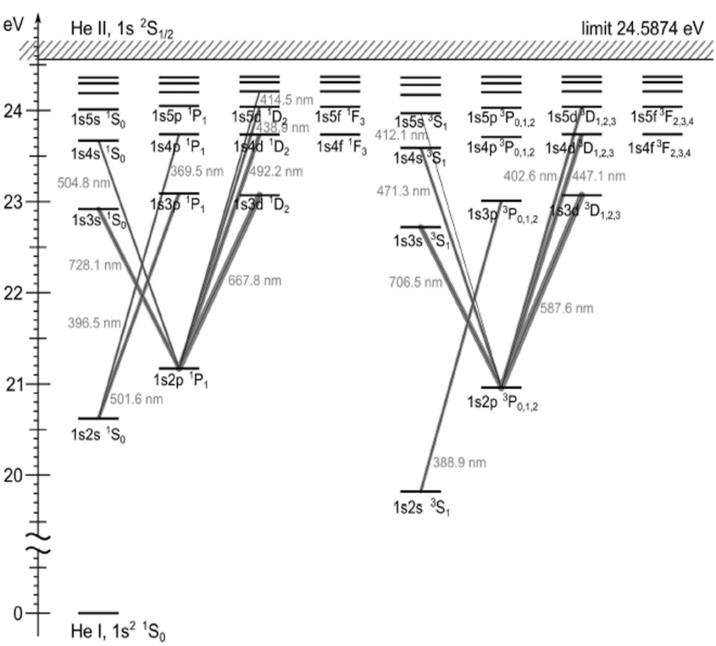
\includegraphics[width=\linewidth]{../plots/he_term_diagram.png}
    \caption{Grotrian term diagram of the neutral helium atom (He I) showing the separate singlet (parahelium, left) and triplet (orthohelium, right) level systems and allowed optical transitions \cite{lab_manual}.}
    \label{fig:term_diagram}
\end{figure}

\subsection{Diffraction Grating Theory}
When monochromatic light of wavelength $\lambda$ falls perpendicularly on a transmission grating with diffraction constant $d$, constructive interference maxima occur at diffraction angles $\theta$ satisfying:
\begin{equation}
    m \lambda = d \sin\theta
    \label{eq:grating_normal}
\end{equation}
where $m = 0, 1, 2, \dots$ is the order number and $d_{\text{manual}} = \SI{1684}{\nano\meter}$ is the accepted manual value for the grating used in this experiment \cite{lab_manual}. By measuring both the left ($\theta_{\text{left}}$) and right ($\theta_{\text{right}}$) goniometer angles relative to the zero-order beam direction $\theta_0$, the average diffraction angle is:
\begin{equation}
    \theta_{\text{ave}} = \frac{|\theta_{\text{left}} - \theta_0| + |\theta_{\text{right}} - \theta_0|}{2}
    \label{eq:theta_ave}
\end{equation}
When the wavelengths $\lambda_{\text{lit}}$ of the observed helium transitions are known from the manual reference spectrum, Equation~\eqref{eq:grating_normal} can be inverted to determine the experimental diffraction grating constant $d$ directly from the measured angles:
\begin{equation}
    d = \frac{m \lambda_{\text{lit}}}{\sin\theta_{\text{ave}}}
    \label{eq:d_from_data}
\end{equation}

% ---------- EXPERIMENTAL SETUP ----------
\section{Experimental Setup}
The spectrometer assembly used to disperse and measure the helium emission spectrum is shown in Figure~\ref{fig:setup}. It comprises the following components \cite{lab_manual, phywe}:
\begin{itemize}
    \item \textbf{Helium Spectral Lamp and Power Supply}: A gas-discharge helium tube excited by electron collisions and powered by a PHYWE spectral-lamp choke/power supply.
    \item \textbf{Collimator}: An optical tube equipped with an adjustable entrance slit and collimating lens to render the incident helium light parallel before reaching the grating.
    \item \textbf{Spectrometer Table and Diffraction Grating}: A rotatable central platform holding a transmission diffraction grating with nominal grating constant $d_{\text{manual}} = \SI{1684}{\nano\meter}$.
    \item \textbf{Goniometer}: A precision circular angular scale with vernier readout ($\pm \SI{0.1}{\degree}$ resolution) centered under the grating table.
    \item \textbf{Observation Telescope (Binoculars)}: An articulated viewing telescope with an internal crosshair used to locate the zero-order image and diffracted spectral lines on both left and right sides.
\end{itemize}

\begin{figure}[H]
    \centering
    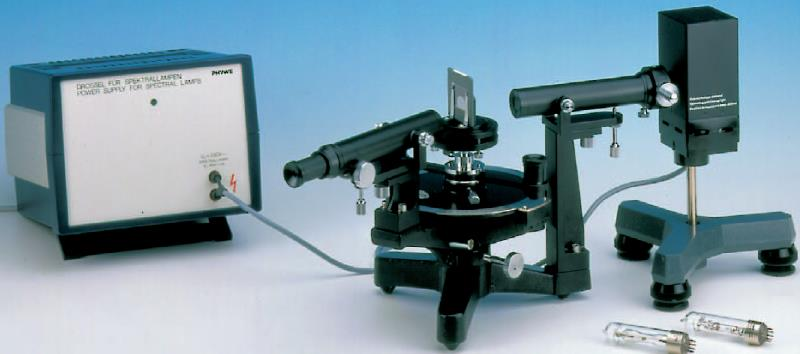
\includegraphics[width=\linewidth]{../plots/he_spectrometer_setup.png}
    \caption{Spectrometer apparatus for analyzing the emission spectrum of helium, showing the spectral-lamp power supply (left), observation telescope and goniometer table with mounted grating (center), collimator, and helium lamp housing (right) \cite{lab_manual}.}
    \label{fig:setup}
\end{figure}

% ---------- PROCEDURE ----------
\section{Experimental Procedure}
The experiment was executed according to the sequence specified in the laboratory manual \cite{lab_manual}:
\begin{enumerate}
    \item The helium spectral lamp was energized and allowed to stabilize so that the visible emission lines appeared sharply through the slit.
    \item The diffraction grating ($d_{\text{manual}} = \SI{1684}{\nano\meter}$) was mounted on the central table and adjusted so that the collimated light struck it perpendicularly.
    \item The observation telescope was centered on the undiffracted zero-order bright line ($m = 0$), and the zero-order angle was read on the goniometer as $\theta_0 = \SI{110.0}{\degree}$.
    \item The telescope was rotated first to the left and then to the right of the central maximum to read $\theta_{\text{left}}$ and $\theta_{\text{right}}$ for each visible first-order ($m = 1$) spectral line (red, yellow, green, blue, and purple). Second-order ($m = 2$) measurements were omitted in this session.
    \item The zero-order angle $\theta_0$ was subtracted from $\theta_{\text{left}}$ and $\theta_{\text{right}}$ to obtain the angular differences $(\theta_{\text{left}} - \theta_0)$ and $(\theta_{\text{right}} - \theta_0)$.
    \item For each spectral color, the average diffraction angle $\theta_{\text{ave}}$ was calculated from the left and right diffraction angles using Equation~\eqref{eq:theta_ave}.
    \item Experimental wavelengths $\lambda_{\text{exp}}$ were calculated for $m = 1$ using Equation~\eqref{eq:grating_normal} with $d_{\text{manual}} = \SI{1684}{\nano\meter}$.
    \item Because only the first diffraction order ($m = 1$) was recorded, averaging wavelengths across $m = 1$ and $m = 2$ was not applicable.
    \item The spectrometer calibration curve was constructed for the values of $\lambda$ and $\sin\theta_{\text{ave}}$ determined at $m = 1$, enabling experimental extraction of the grating constant $d$ for comparison with $d_{\text{manual}}$.
\end{enumerate}

% ---------- DATA ANALYSIS ----------
\section{Data Analysis}

\subsection{Diffraction Angle Reduction and Wavelength Determination (\texorpdfstring{$d_{\text{manual}} = \SI{1684}{\nano\meter}$}{d\_manual = 1684 nm})}
For every observed spectral line, $\theta_{\text{left}} < \theta_0 < \theta_{\text{right}}$, so Equation~\eqref{eq:theta_ave} reduces algebraically to $\theta_{\text{ave}} = (\theta_{\text{right}} - \theta_{\text{left}})/2$, canceling any uniform offset in $\theta_0$. Using the red line ($\theta_{\text{left}} = \SI{88.0}{\degree}$, $\theta_{\text{right}} = \SI{139.9}{\degree}$) as a representative example:
\begin{equation}
\begin{aligned}
    \theta_{\text{ave, red}} &= \frac{|88.0 - 110.0| + |139.9 - 110.0|}{2} \\
    &= \frac{22.0 + 29.9}{2} = \SI{25.95}{\degree}
\end{aligned}
    \label{eq:example_theta_ave}
\end{equation}
Applying Equation~\eqref{eq:grating_normal} with $m = 1$ and $d_{\text{manual}} = \SI{1684.0}{\nano\meter}$ gives:
\begin{equation}
    \lambda(d_{\text{manual}})_{\text{red}} = \SI{1684.0}{\nano\meter} \times \sin(\SI{25.95}{\degree}) = \SI{736.9}{\nano\meter}
    \label{eq:example_lambda}
\end{equation}

Propagating independent goniometer reading uncertainties of $\sigma_\theta = \SI{0.1}{\degree}$ for $\theta_{\text{left}}$ and $\theta_{\text{right}}$ yields:
\begin{equation}
    \sigma_{\theta_{\text{ave}}} = \frac{\sigma_\theta}{\sqrt{2}} = \SI{0.0707}{\degree}, \qquad \sigma_\lambda = \frac{d}{m} \cos\theta_{\text{ave}}\,\sigma_{\theta_{\text{ave}}}
    \label{eq:error_prop}
\end{equation}
with $\sigma_{\theta_{\text{ave}}}$ expressed in radians inside Equation~\eqref{eq:error_prop}. Using $d_{\text{manual}} = \SI{1684.0}{\nano\meter}$, $\sigma_\lambda$ ranges from $\SI{1.87}{\nano\meter}$ (red) to $\SI{2.00}{\nano\meter}$ (purple). Matching the five observed colors to the brightest allowed helium transitions in Tables~1 and 2 of the manual \cite{lab_manual} assigns: red ($3\,^{1}D \rightarrow 2\,^{1}P$, singlet, $\lambda_{\text{lit}} = \SI{667.8}{\nano\meter}$), yellow ($3\,^{3}D \rightarrow 2\,^{3}P$, triplet, $\SI{587.6}{\nano\meter}$), green ($4\,^{1}S \rightarrow 2\,^{1}P$, singlet, $\SI{504.8}{\nano\meter}$), blue ($4\,^{3}D \rightarrow 2\,^{3}P$, triplet, $\SI{447.1}{\nano\meter}$), and purple ($3\,^{3}P \rightarrow 2\,^{3}S$, triplet, $\SI{388.9}{\nano\meter}$). Across all five lines, $\lambda(d_{\text{manual}})$ systematically exceeds $\lambda_{\text{lit}}$ by a mean offset of $+\SI{69.24}{\nano\meter}$, yielding relative errors between \SI{10.35}{\percent} and \SI{15.72}{\percent} (mean \SI{13.66}{\percent}).

\subsection{Experimental Determination of the Grating Constant \texorpdfstring{$d$}{d}}
Using the accepted manual wavelengths $\lambda_{\text{lit}}$ and the measured $\sin\theta_{\text{ave}}$ values at $m = 1$, Equation~\eqref{eq:d_from_data} yields an experimental grating constant $d_i$ for each observed spectral line. For the red line ($\lambda_{\text{lit}} = \SI{667.8}{\nano\meter}$, $\sin\theta_{\text{ave}} = 0.4376$):
\begin{equation}
    d_{\text{red}} = \frac{1 \times \SI{667.8}{\nano\meter}}{\sin(\SI{25.95}{\degree})} = \SI{1526.1}{\nano\meter}
    \label{eq:example_d_calc}
\end{equation}
The reading uncertainty $\sigma_{d_i}$ propagated from $\sigma_{\theta_{\text{ave}}}$ via Equation~\eqref{eq:d_from_data} is:
\begin{equation}
    \sigma_{d_i} = \frac{m \lambda_{\text{lit},i} \cos\theta_{\text{ave},i}}{\sin^2\theta_{\text{ave},i}}\,\sigma_{\theta_{\text{ave}}}
    \label{eq:sigma_d_calc}
\end{equation}
giving values between $\SI{3.9}{\nano\meter}$ (red) and $\SI{6.5}{\nano\meter}$ (purple). Across all five spectral lines, $d_i$ spans $\SI{1455.3}{\nano\meter}$ to $\SI{1526.1}{\nano\meter}$, with an arithmetic mean and standard error of:
\begin{equation}
    \bar{d} = \SI{1482.0 \pm 12.9}{\nano\meter} \quad (s_d = \SI{28.8}{\nano\meter})
    \label{eq:d_bar}
\end{equation}
This experimental mean differs from the accepted manual value $d_{\text{manual}} = \SI{1684.0}{\nano\meter}$ by \SI{11.99}{\percent}. Re-evaluating the spectral wavelengths via Equation~\eqref{eq:grating_normal} with $d = \bar{d}$ (and propagating combined uncertainty from $\sigma_{\theta_{\text{ave}}}$ and $\sigma_{\bar{d}}$) yields $\lambda(\bar{d})$ values ranging from $\SI{396.1 \pm 3.9}{\nano\meter}$ (purple) to $\SI{648.5 \pm 5.9}{\nano\meter}$ (red), lowering the relative wavelength error against the accepted manual reference values to between \SI{0.23}{\percent} (blue) and \SI{2.89}{\percent} (red), with a mean relative error of \SI{1.44}{\percent}.

\subsection{Spectrometer Calibration Curve (\texorpdfstring{$m = 1$}{m = 1})}
Following Step~9 of the manual, the $m = 1$ calibration curve was constructed by performing ordinary least-squares (OLS) linear regression between $\lambda_{\text{lit}}$ and $\sin\theta_{\text{ave}}$:
\begin{equation}
    \lambda_{\text{lit}} = d_{\text{cal}} \sin\theta_{\text{ave}} + b
    \label{eq:calibration_ols}
\end{equation}
Unconstrained OLS regression yielded a calibrated slope of $d_{\text{cal}} = \SI{1617.1 \pm 52.3}{\nano\meter}$ and an intercept of $b = \SI{-45.9 \pm 18.6}{\nano\meter}$, with $R^2 = 0.9969$ ($p = \SI{7.446e-5}{}$) and a root-mean-square (RMS) residual of $\SI{5.55}{\nano\meter}$. The unconstrained slope $d_{\text{cal}}$ agrees within \SI{3.97}{\percent} of $d_{\text{manual}} = \SI{1684.0}{\nano\meter}$. In inverse form, the linear fit gives $\sin\theta_{\text{ave}} = (6.164 \pm 0.199) \times 10^{-4}\,\mathrm{nm^{-1}}\,\lambda_{\text{lit}} + (0.0294 \pm 0.0105)$. Performing a zero-intercept proportionality fit ($\lambda_{\text{lit}} = d_{\text{eff}} \sin\theta_{\text{ave}}$) directly constrained to Equation~\eqref{eq:grating_normal} produced an effective grating constant of $d_{\text{eff}} = \SI{1489.8 \pm 13.6}{\nano\meter}$ ($R^2 = 0.9905$, RMS residual $\SI{9.66}{\nano\meter}$), differing from $d_{\text{manual}}$ by \SI{11.53}{\percent} and closely matching $\bar{d}$.

% ---------- RESULTS ----------
\section{Results}

\subsection{Tabulated Experimental Data and Comparisons}
The first-order ($m = 1$) goniometer readings, angular differences, average diffraction angles, and wavelengths obtained with $d_{\text{manual}} = \SI{1684.0}{\nano\meter}$ are presented in Table~\ref{tab:m1_results}, following the structure of Table~3 in the manual. Table~\ref{tab:lit_comparison} compares the wavelengths calculated from $d_{\text{manual}}$, the line-by-line experimental grating constants $d_i$, and the $\bar{d}$-calibrated wavelengths against the accepted manual reference lines. Table~\ref{tab:calibration_summary} summarizes all experimentally determined grating constants and calibration metrics against $d_{\text{manual}} = \SI{1684.0}{\nano\meter}$.

\begin{table*}[t]
    \centering
    \caption{First-Order ($m = 1$) Diffraction Angles and Experimental Wavelengths Using $d_{\text{manual}} = \SI{1684.0}{\nano\meter}$ ($\theta_0 = \SI{110.0}{\degree}$)}
    \label{tab:m1_results}
    \pgfplotstabletypeset[
        string type,
        columns={Color,theta_0,theta_left,diff_left,theta_right,diff_right,theta_ave,sin_theta_ave,lambda_exp},
        columns/Color/.style={column name=\textbf{Color}},
        columns/theta_0/.style={column name=$\mathbf{\theta_0}$ (\si{\degree})},
        columns/theta_left/.style={column name=$\mathbf{\theta_{\text{left}}}$ (\si{\degree})},
        columns/diff_left/.style={column name=$\mathbf{(\theta_{\text{left}}-\theta_0)}$ (\si{\degree})},
        columns/theta_right/.style={column name=$\mathbf{\theta_{\text{right}}}$ (\si{\degree})},
        columns/diff_right/.style={column name=$\mathbf{(\theta_{\text{right}}-\theta_0)}$ (\si{\degree})},
        columns/theta_ave/.style={column name=$\mathbf{\theta_{\text{ave}}}$ (\si{\degree})},
        columns/sin_theta_ave/.style={column name=$\mathbf{\sin\theta_{\text{ave}}}$},
        columns/lambda_exp/.style={column name=$\mathbf{\lambda(d_{\text{man}})}$ (\si{\nano\meter})}
    ]{tables/table1_m1_results.csv}
\end{table*}

\begin{table*}[t]
    \centering
    \caption{Comparison of Experimental Wavelengths and Calculated Grating Constants $d_i$ Against Accepted Manual Values}
    \label{tab:lit_comparison}
    \pgfplotstabletypeset[
        string type,
        columns={Color,Transition,System,lambda_lit,lambda_man,err_man_pct,d_calc,lambda_dbar,err_dbar_pct},
        columns/Color/.style={column name=\textbf{Color}},
        columns/Transition/.style={column name=\textbf{Transition}},
        columns/System/.style={column name=\textbf{System}},
        columns/lambda_lit/.style={column name=$\mathbf{\lambda_{\text{lit}}}$ (\si{\nano\meter})},
        columns/lambda_man/.style={column name=$\mathbf{\lambda(d_{\text{man}})}$ (\si{\nano\meter})},
        columns/err_man_pct/.style={column name=\textbf{Err. ($d_{\text{man}}$) \%}},
        columns/d_calc/.style={column name=$\mathbf{d_i}$ (\si{\nano\meter})},
        columns/lambda_dbar/.style={column name=$\mathbf{\lambda(\bar{d})}$ (\si{\nano\meter})},
        columns/err_dbar_pct/.style={column name=\textbf{Err. ($\bar{d}$) \%}}
    ]{tables/table2_literature_comparison.csv}
\end{table*}

\begin{table}[H]
    \centering
    \caption{Comparison of Experimental Grating Constants and Calibration Metrics Against the Accepted Manual Value}
    \label{tab:calibration_summary}
    \resizebox{\columnwidth}{!}{%
    \pgfplotstabletypeset[
        string type,
        columns={Parameter,Value,Unit,Diff_vs_Manual},
        columns/Parameter/.style={column name=\textbf{Parameter}},
        columns/Value/.style={column name=\textbf{Value}},
        columns/Unit/.style={column name=\textbf{Unit}},
        columns/Diff_vs_Manual/.style={column name=\textbf{Diff. vs. Manual}}
    ]{tables/table3_calibration_summary.csv}%
    }
\end{table}

\subsection{Graphical Analysis}
The $m = 1$ spectrometer calibration curve is shown in Figure~\ref{fig:calibration}, comparing the manual grating equation $\lambda = 1684\sin\theta_{\text{ave}}$ against the unconstrained OLS calibration line ($R^2 = 0.9969$) and the zero-intercept fit ($d_{\text{eff}} = \SI{1489.8 \pm 13.6}{\nano\meter}$). Figure~\ref{fig:grating_comparison} displays the line-by-line grating constants $d_i$, their sample mean $\bar{d} = \SI{1482.0 \pm 12.9}{\nano\meter}$, and the OLS calibration slope $d_{\text{cal}} = \SI{1617.1 \pm 52.3}{\nano\meter}$ relative to the manual value $d_{\text{manual}} = \SI{1684.0}{\nano\meter}$. Finally, Figure~\ref{fig:wavelength_comparison} compares the wavelengths obtained using $d_{\text{manual}}$ and $\bar{d}$ against the accepted manual reference wavelengths across the visible helium spectrum.

\begin{figure}[H]
    \centering
    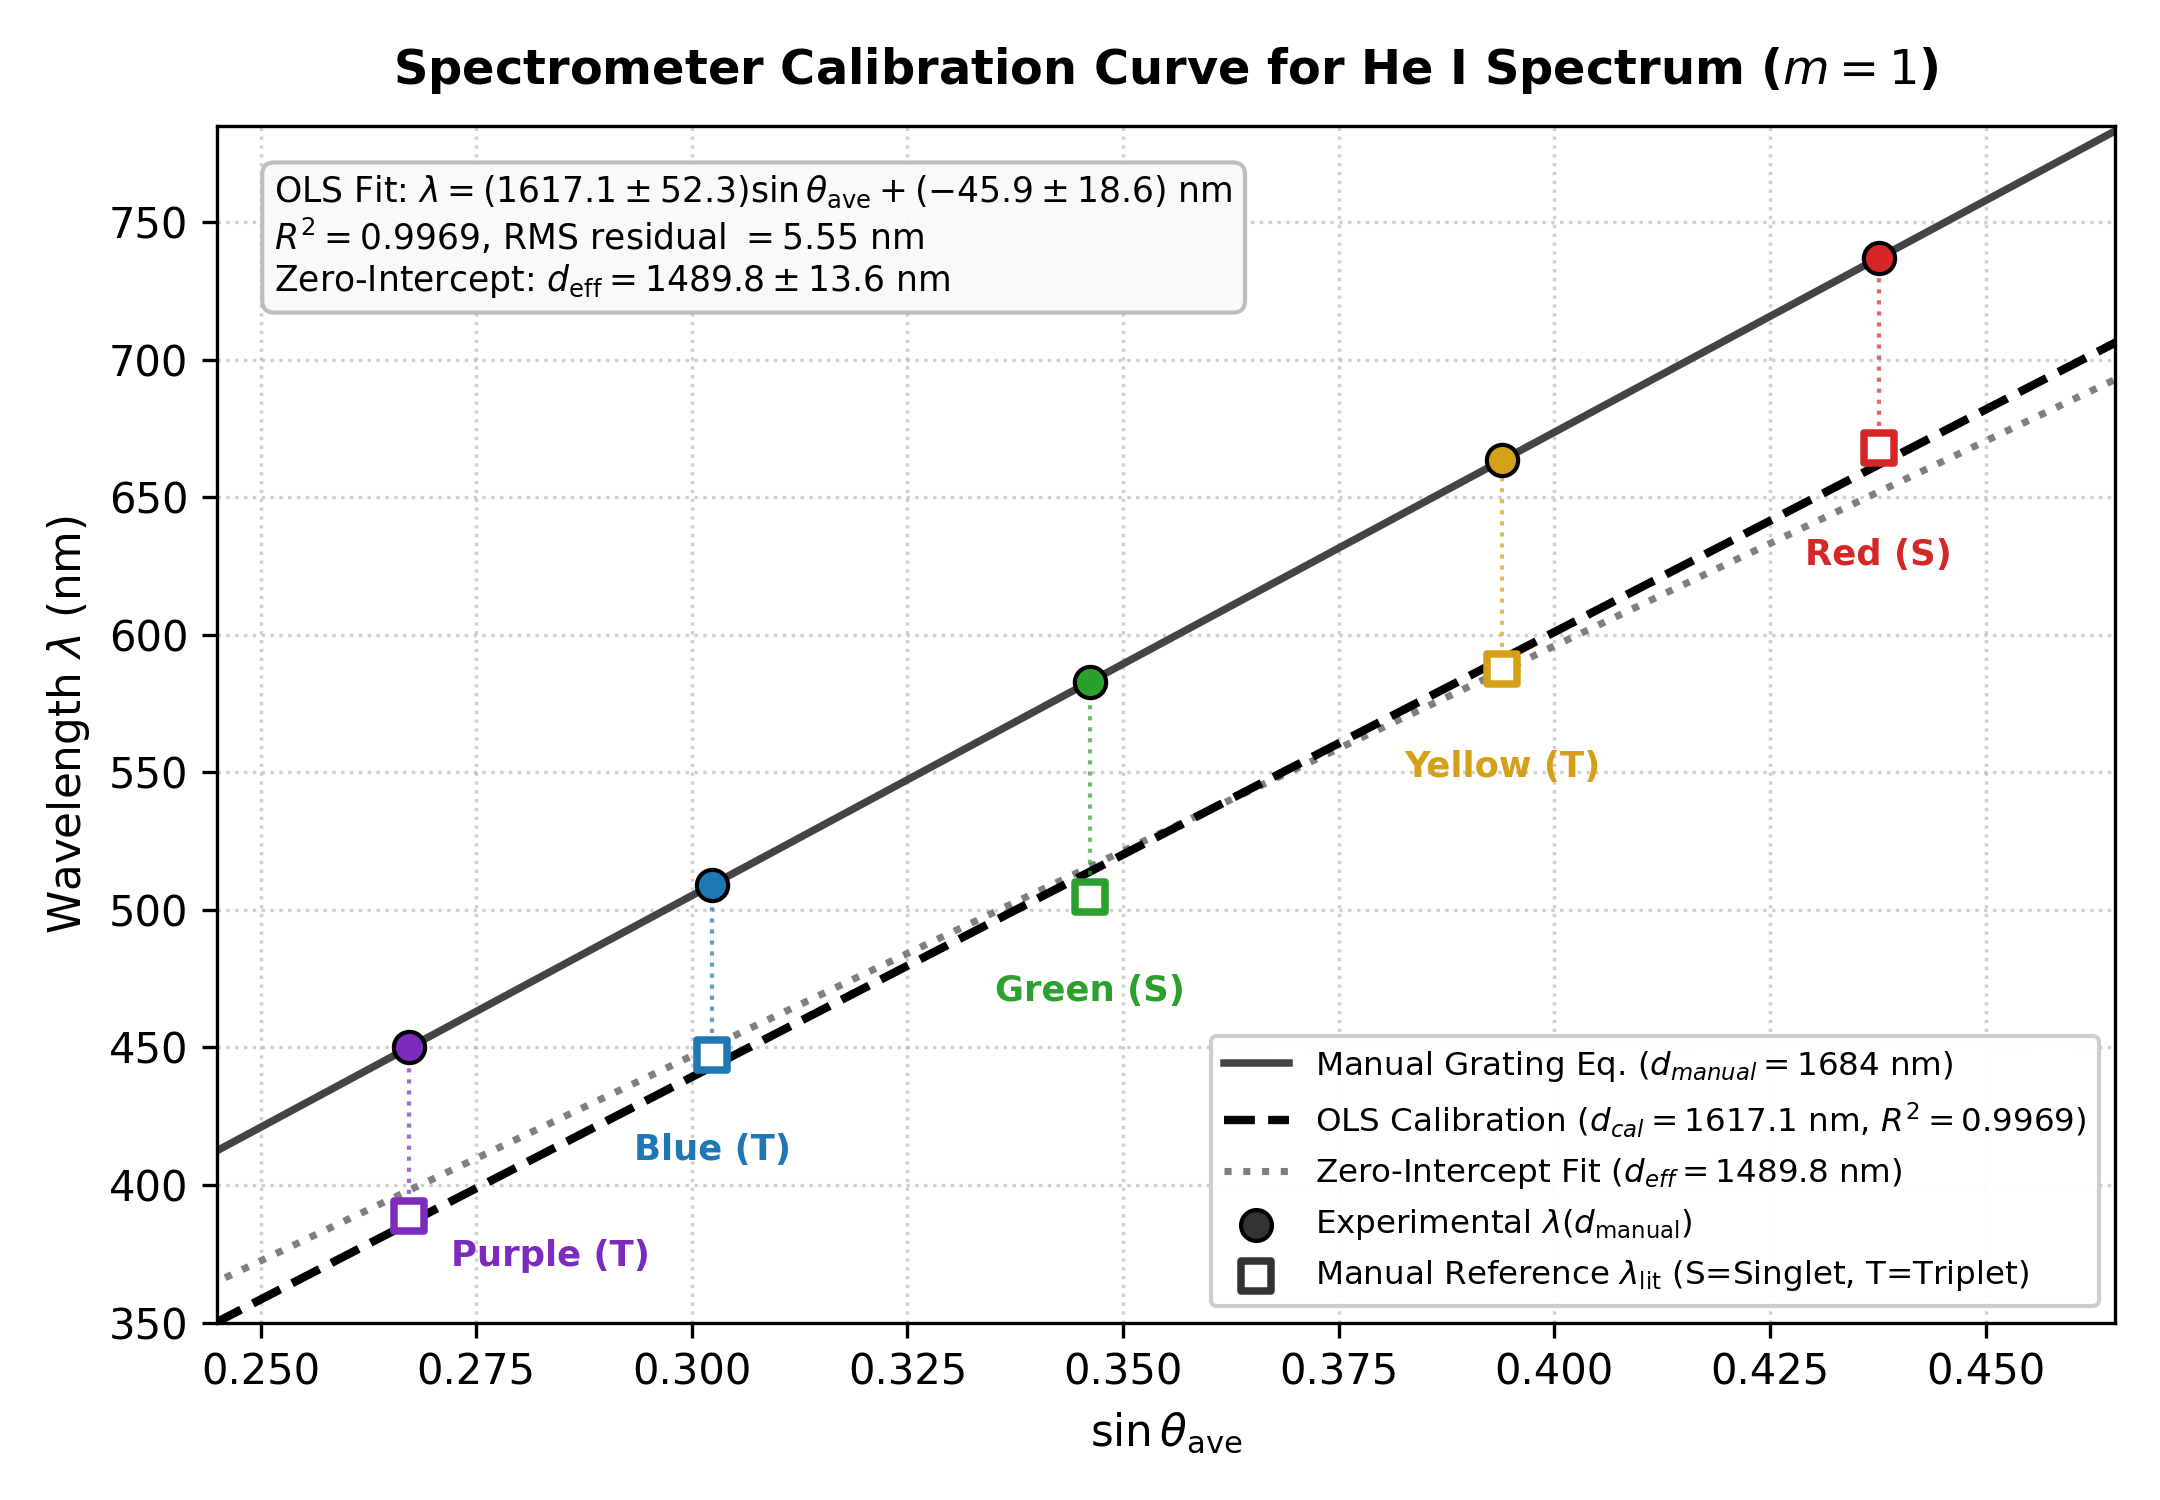
\includegraphics[width=\linewidth]{../plots/calibration_curve_m1.png}
    \caption{Spectrometer calibration curve for $m = 1$ relating $\lambda$ to $\sin\theta_{\text{ave}}$. Solid circles denote experimental wavelengths evaluated with $d_{\text{manual}} = \SI{1684}{\nano\meter}$, and open squares indicate accepted manual wavelengths fitted by unconstrained OLS ($R^2 = 0.9969$) and zero-intercept proportionality.}
    \label{fig:calibration}
\end{figure}

\begin{figure}[H]
    \centering
    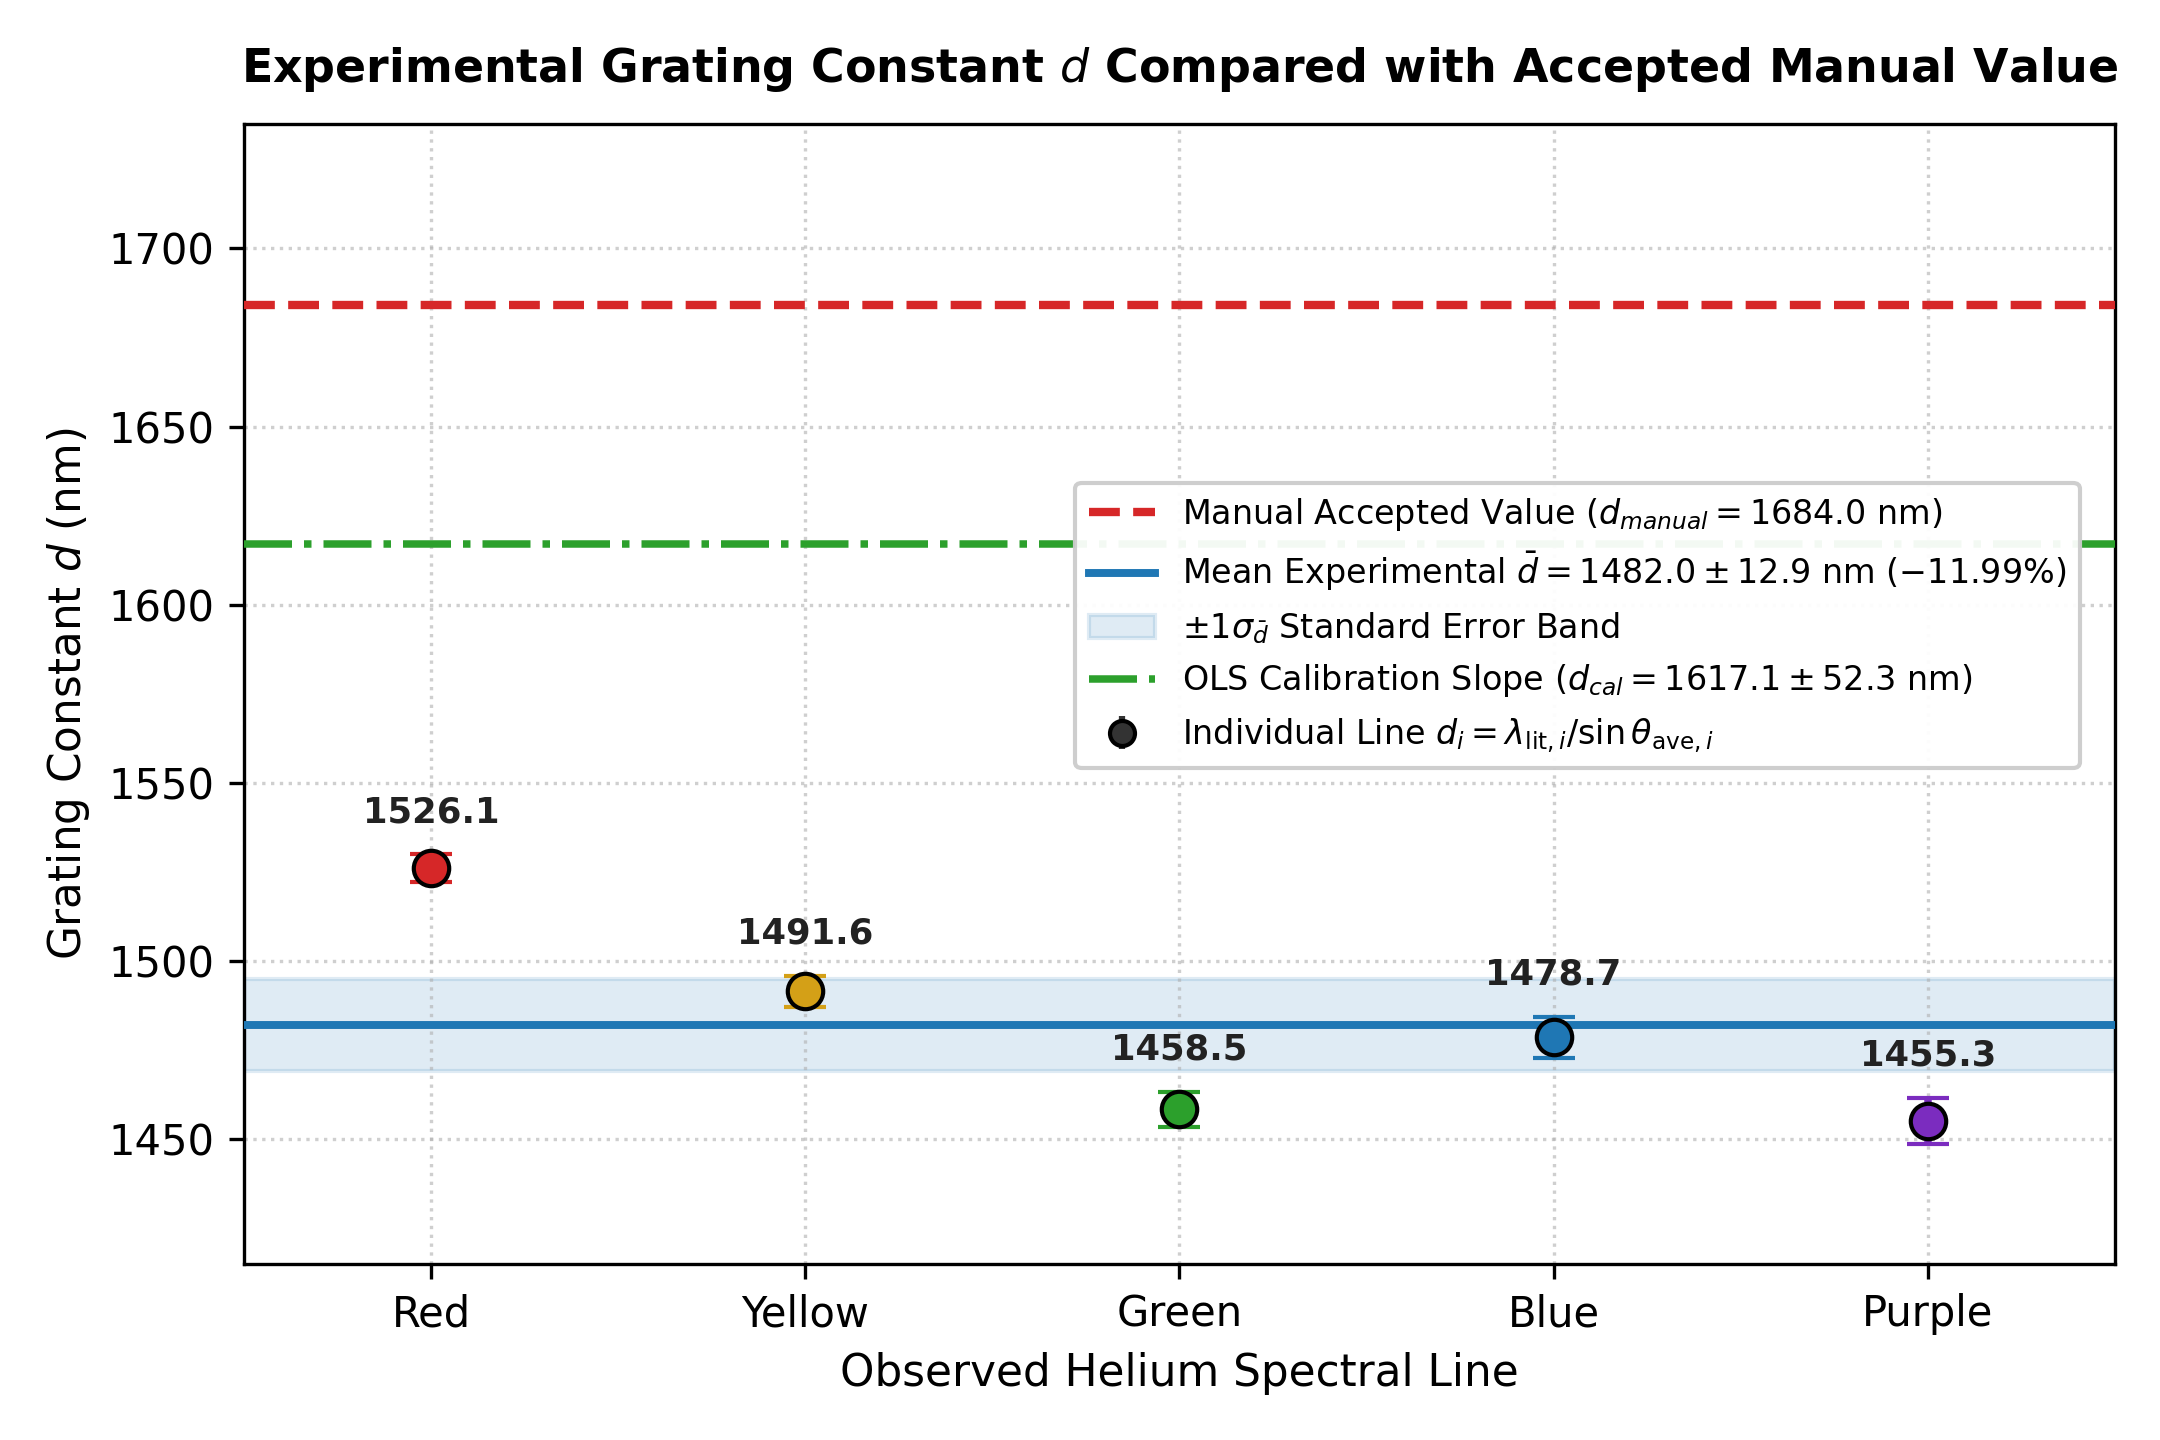
\includegraphics[width=\linewidth]{../plots/grating_constant_comparison.png}
    \caption{Line-by-line experimental grating constants $d_i = \lambda_{\text{lit},i}/\sin\theta_{\text{ave},i}$ with propagated reading uncertainties compared against the mean $\bar{d} = \SI{1482.0 \pm 12.9}{\nano\meter}$, OLS calibration slope $d_{\text{cal}} = \SI{1617.1 \pm 52.3}{\nano\meter}$, and accepted manual value $d_{\text{manual}} = \SI{1684.0}{\nano\meter}$.}
    \label{fig:grating_comparison}
\end{figure}

\begin{figure}[H]
    \centering
    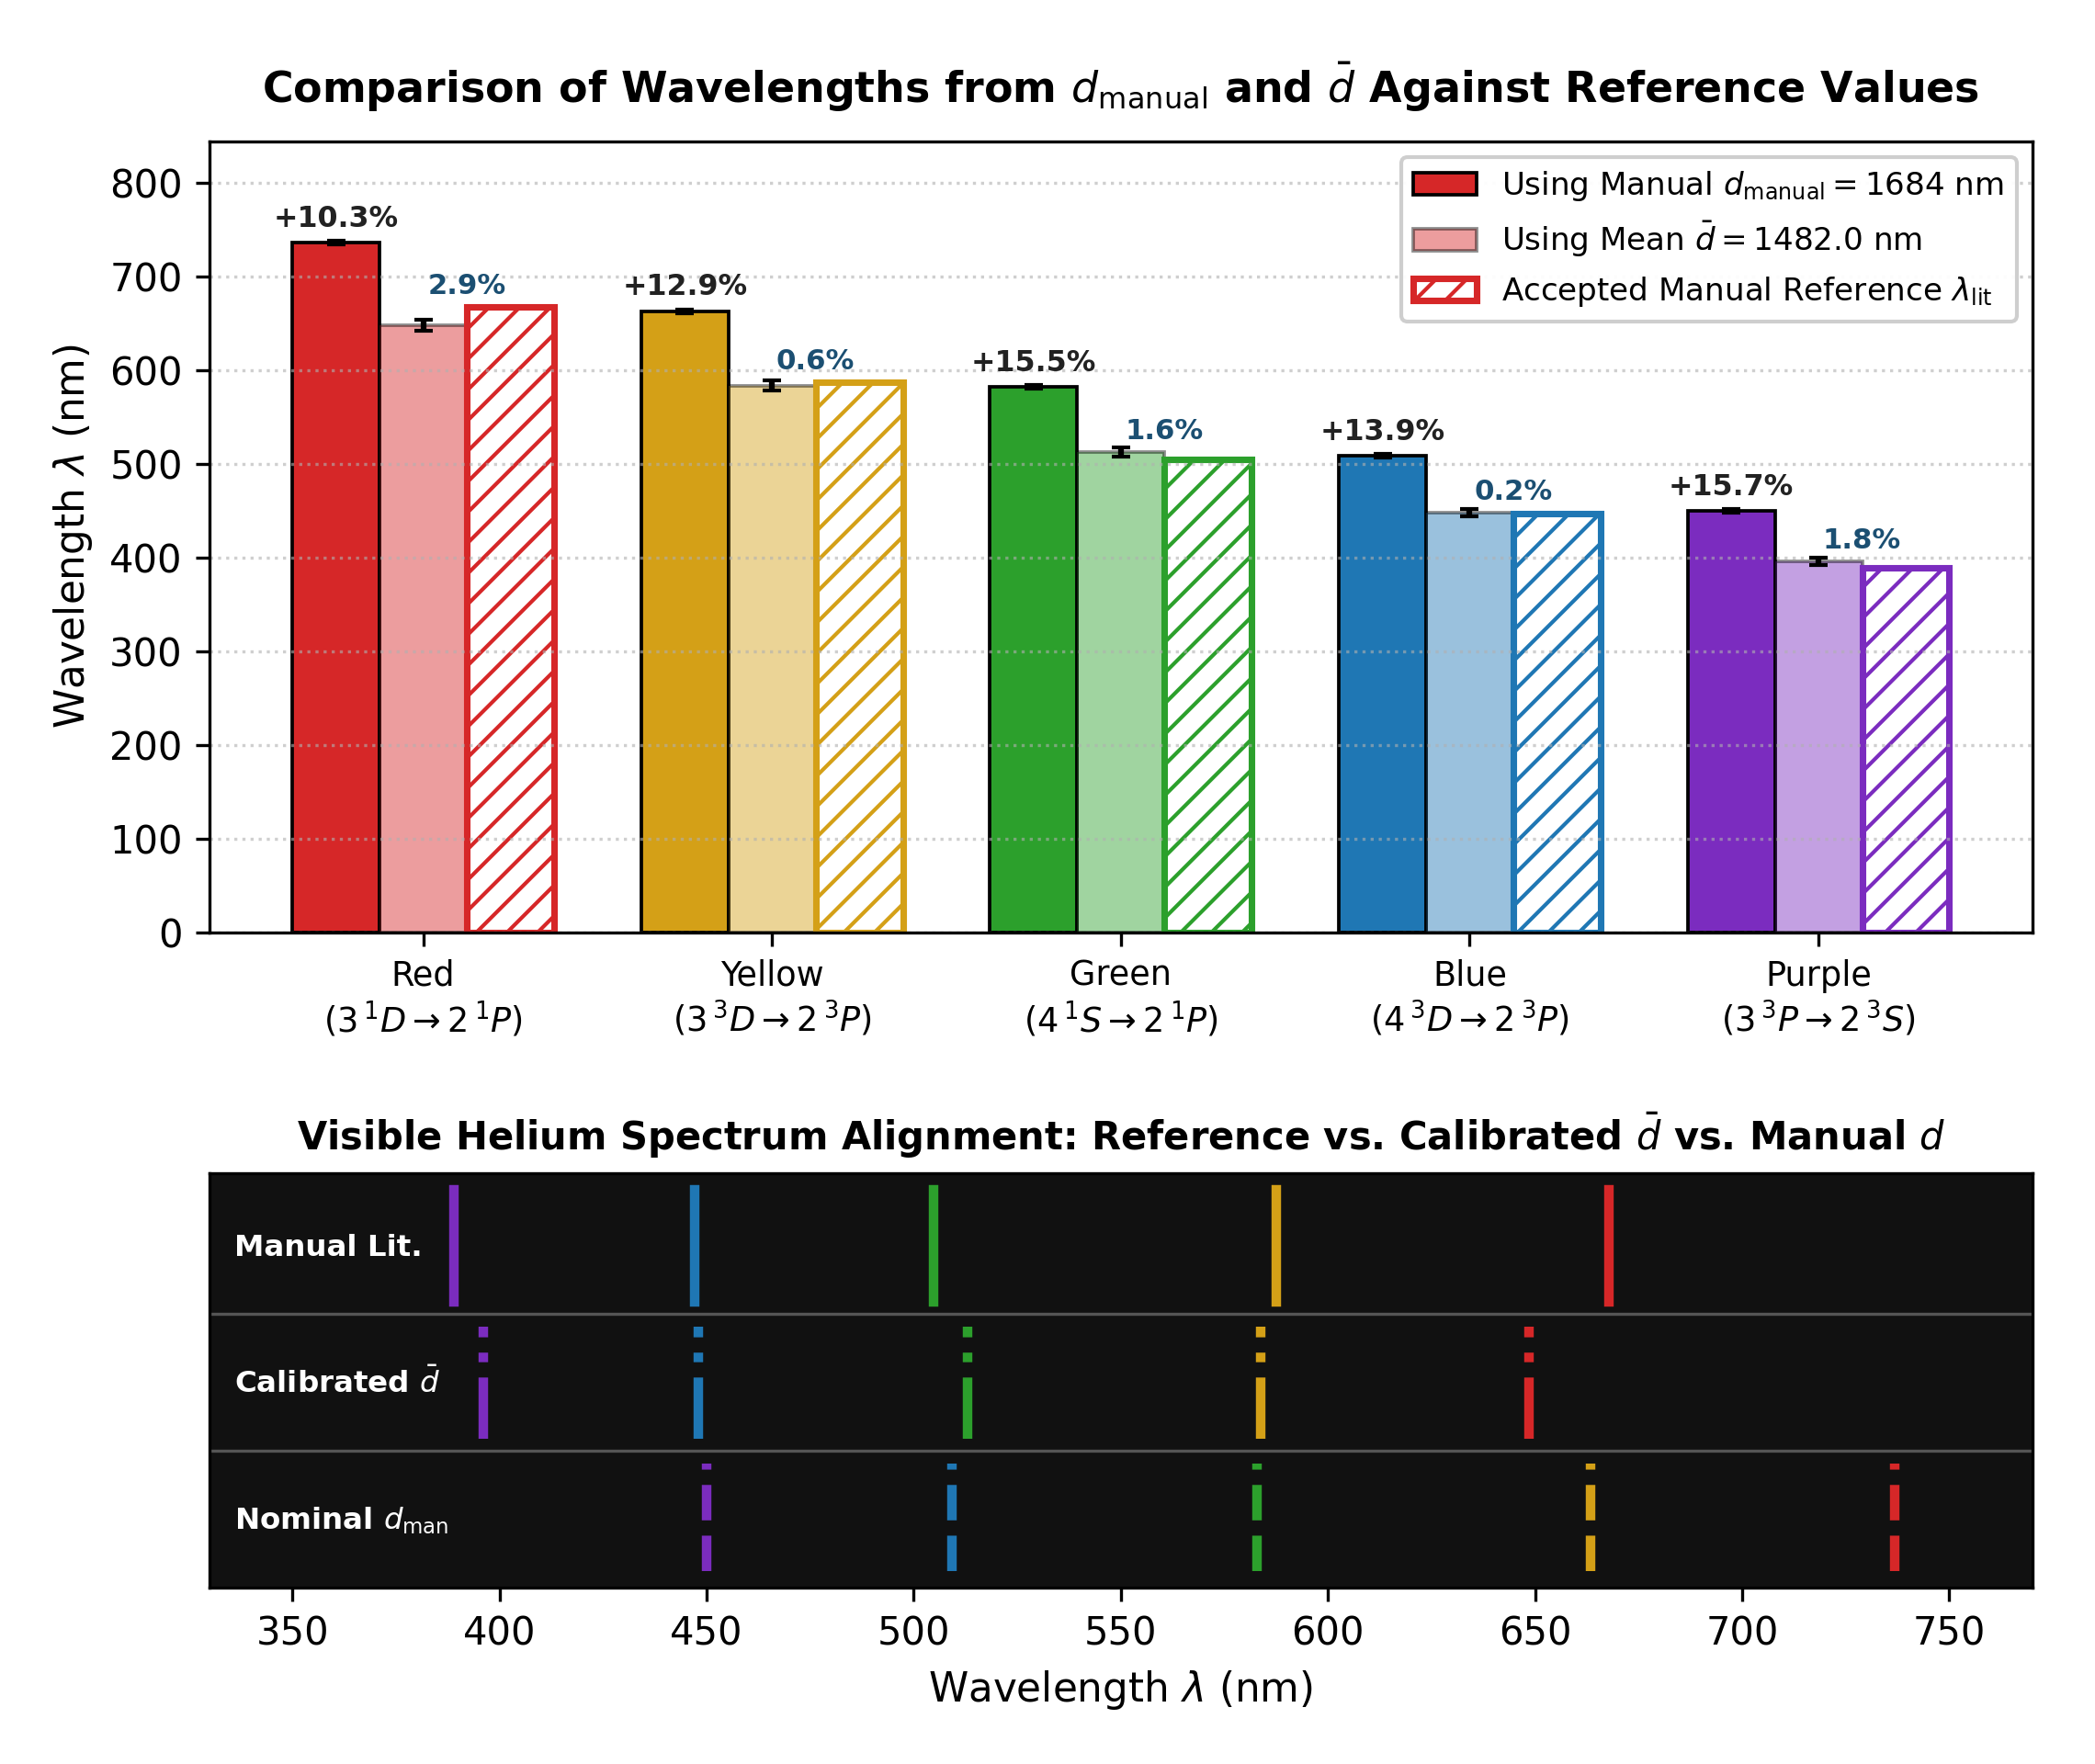
\includegraphics[width=\linewidth]{../plots/wavelength_comparison.png}
    \caption{Top: Comparison of wavelengths computed using $d_{\text{manual}}$ and calibrated $\bar{d}$ against accepted manual reference wavelengths. Bottom: Visible helium spectrum alignment showing how applying $\bar{d}$ brings all five lines within \SI{1.44}{\percent} mean error of the reference spectrum.}
    \label{fig:wavelength_comparison}
\end{figure}

% ---------- DISCUSSION ----------
\section{Discussion}

\subsection{Identification of Singlet and Triplet Transitions}
The five observed spectral lines span both non-combining term manifolds of He I: the red ($\SI{667.8}{\nano\meter}$, $3\,^{1}D \rightarrow 2\,^{1}P$) and green ($\SI{504.8}{\nano\meter}$, $4\,^{1}S \rightarrow 2\,^{1}P$) lines belong to the parahelium singlet system ($S = 0$), whereas the yellow ($\SI{587.6}{\nano\meter}$, $3\,^{3}D \rightarrow 2\,^{3}P$), blue ($\SI{447.1}{\nano\meter}$, $4\,^{3}D \rightarrow 2\,^{3}P$), and purple ($\SI{388.9}{\nano\meter}$, $3\,^{3}P \rightarrow 2\,^{3}S$) lines belong to the orthohelium triplet system ($S = 1$) \cite{lab_manual}. Although the $2\,^{3}P_{0,1,2}$ and $3\,^{3}D_{1,2,3}$ triplet terms exhibit genuine fine-structure splitting from the spin-orbit term in Equation~\eqref{eq:hamiltonian}, the energy separations between adjacent $J$ sublevels in helium are typically $\SI{e-5}{\electronvolt}$ to $\SI{e-4}{\electronvolt}$ (wavelength splittings below $\SI{0.1}{\nano\meter}$) \cite{haken_wolf, svanberg}. Because the first-order dispersion of the diffraction grating yields a vernier-limited wavelength resolution of $\sigma_\lambda \approx \SI{1.9}{\nano\meter}$, each triplet multiplet appears as a single unresolved spectral line in the telescope. Furthermore, Table~2 of the manual lists two green lines ($\SI{504.8}{\nano\meter}$ and $\SI{492.2}{\nano\meter}$); the weak singlet line at $\SI{504.8}{\nano\meter}$ (relative intensity 2) is especially sensitive to visual crosshair centering under dim illumination.

\subsection{Comparison with Accepted Manual Values and Error Analysis}
Comparing the experimentally extracted grating constants against the manual's accepted value $d_{\text{manual}} = \SI{1684.0}{\nano\meter}$ highlights two complementary findings (Table~\ref{tab:calibration_summary} and Figure~\ref{fig:grating_comparison}):
\begin{enumerate}
    \item \textbf{Calibration Slope vs. Mean Effective Constant}: The unconstrained OLS calibration slope $d_{\text{cal}} = \SI{1617.1 \pm 52.3}{\nano\meter}$ ($R^2 = 0.9969$) agrees closely with $d_{\text{manual}} = \SI{1684.0}{\nano\meter}$ within \SI{3.97}{\percent} (just over $1.2\sigma$), confirming that the spectrometer dispersion follows the linear proportionality of Equation~\eqref{eq:grating_normal} across the visible spectrum. By contrast, the non-zero intercept $b = \SI{-45.9 \pm 18.6}{\nano\meter}$ shifts the line-by-line average $\bar{d} = \SI{1482.0 \pm 12.9}{\nano\meter}$ (\SI{11.99}{\percent} difference) and zero-intercept fit $d_{\text{eff}} = \SI{1489.8 \pm 13.6}{\nano\meter}$ (\SI{11.53}{\percent} difference) systematically below $d_{\text{manual}}$.
    \item \textbf{Wavelength Comparison ($d_{\text{manual}}$ vs. $\bar{d}$)}: Using $d_{\text{manual}}$ produces an almost constant positive offset ($\overline{\Delta\lambda} = +\SI{69.24}{\nano\meter}$, mean error \SI{13.66}{\percent}), whereas evaluating $\lambda = \bar{d}\sin\theta_{\text{ave}}$ reduces the mean wavelength discrepancy to \SI{1.44}{\percent} (Figure~\ref{fig:wavelength_comparison}).
    \item \textbf{Sources of Systematic and Random Error}: Inspection of Table~\ref{tab:m1_results} shows two physical signatures within the experimental procedure: first, the midpoint of the left and right readings $(\theta_{\text{left}} + \theta_{\text{right}})/2$ averages $\SI{113.26 \pm 0.54}{\degree}$ rather than the recorded zero-order angle $\theta_0 = \SI{110.0}{\degree}$; second, the right-side deflections $|\theta_{\text{right}} - \theta_0|$ consistently exceed the left-side deflections $|\theta_{\text{left}} - \theta_0|$ by $\SI{6.52 \pm 1.07}{\degree}$. This asymmetry indicates that the grating was not positioned strictly perpendicular to the collimated light beam during Step~2 of the procedure and that the zero-order reference reading ($\theta_0 = \SI{110.0}{\degree}$) contained a slight alignment offset. In addition, the actual ruling spacing of the mounted grating may differ slightly from the nominal value printed in the manual. Random errors arise from the $\pm \SI{0.1}{\degree}$ goniometer vernier resolution, finite collimator slit width, visual centering on faint lines, and the omission of second-order ($m = 2$) measurements, which prevented higher-dispersion averaging across orders.
\end{enumerate}

% ---------- CONCLUSION ----------
\section{Conclusion}
First-order ($m = 1$) diffraction measurements of the visible He I emission spectrum were performed using a grating spectrometer ($\theta_0 = \SI{110.0}{\degree}$). Evaluating the observed spectral lines with the accepted manual grating constant $d_{\text{manual}} = \SI{1684.0}{\nano\meter}$ yielded wavelengths of $\SI{736.9 \pm 1.9}{\nano\meter}$ (red), $\SI{663.4 \pm 1.9}{\nano\meter}$ (yellow), $\SI{582.9 \pm 1.9}{\nano\meter}$ (green), $\SI{509.2 \pm 2.0}{\nano\meter}$ (blue), and $\SI{450.0 \pm 2.0}{\nano\meter}$ (purple), with a mean relative error of \SI{13.66}{\percent} compared to the manual's parahelium singlet ($3\,^{1}D \rightarrow 2\,^{1}P$, $4\,^{1}S \rightarrow 2\,^{1}P$) and orthohelium triplet ($3\,^{3}D \rightarrow 2\,^{3}P$, $4\,^{3}D \rightarrow 2\,^{3}P$, $3\,^{3}P \rightarrow 2\,^{3}S$) reference lines. Determining the grating constant directly from the data gave a line-by-line mean of $\bar{d} = \SI{1482.0 \pm 12.9}{\nano\meter}$ (\SI{11.99}{\percent} difference from $d_{\text{manual}}$), an unconstrained calibration slope of $d_{\text{cal}} = \SI{1617.1 \pm 52.3}{\nano\meter}$ ($R^2 = 0.9969$, \SI{3.97}{\percent} difference from $d_{\text{manual}}$), and a zero-intercept slope of $d_{\text{eff}} = \SI{1489.8 \pm 13.6}{\nano\meter}$ (\SI{11.53}{\percent} difference). Re-evaluating the spectrum with the calibrated mean $\bar{d}$ lowered the mean relative wavelength discrepancy to \SI{1.44}{\percent}, confirming the linear grating dispersion law and the non-combining singlet and triplet energy structure of helium.

% ---------- ADDITIONAL RESOURCES ----------
\section{Additional Resources}
Complete computational notebooks, data processing pipelines, and related experimental laboratory reports are maintained in the GitHub repository.

\begin{figure}[H]
    \centering
    \begin{minipage}{0.15\textwidth}
        \centering
        \qrcode[height=1.5cm]{https://github.com/ibeuler/LAB-Reports.git}
    \end{minipage}%
    \begin{minipage}{0.2\textwidth}
        \raggedright
        \caption{Scan QR code to access the GitHub repository containing analysis code and data.}
        \label{fig:qr_code}
    \end{minipage}
\end{figure}

\begin{thebibliography}{9}
\bibitem{lab_manual}
    ISTANBUL UNIVERSITY, \textit{06-FINE STRUCTURE of TWO-ELECTRON ATOM He Laboratory Manual}, Department of Physics, 2026.
\bibitem{haken_wolf}
    H. Haken and H. C. Wolf, \textit{The Physics of Atoms and Quanta}, Springer, 2000.
\bibitem{phywe}
    Phywe Systeme GmbH, \textit{Experimental Literature and Operating Manuals}, G\"ottingen, Germany.
\bibitem{hyperphysics}
    C. R. Nave, ``Helium Energy Levels and Spectra,'' \textit{HyperPhysics}, Georgia State University. [Online]. Available: \url{http://hyperphysics.phy-astr.gsu.edu}
\bibitem{svanberg}
    S. Svanberg, \textit{Atomic and Molecular Spectroscopy: Basic Aspects and Practical Applications}, Springer, 2001.
\end{thebibliography}

\end{document}
